\documentclass[mathserif,serif]{beamer}
\usetheme{Madrid}
\usecolortheme{seagull}
\beamertemplatenavigationsymbolsempty

\usepackage{graphicx}
\usepackage{amsfonts}
\usepackage{courier}

\usepackage{fancyvrb}
\fvset{commandchars=\\\{\}}

\newenvironment{items}{
\begin{itemize}
  \setlength{\itemsep}{0pt}
  \setlength{\parskip}{7pt}
  \setlength{\parsep}{4pt}
}{\end{itemize}}

\title{A Quantitative Analysis of Errors in Linux}
\subtitle{Elvis Flesborg \\ @ Helenekilde Badehotel, Tisvildeleje}

\begin{document}

\frame{\titlepage}

\begin{frame}[t]
    \frametitle{About Me}

    \begin{items}
        \item Elvis Flesborg
        \item Master thesis at IT University of Copenhagen
        \item Specialization in scalable computing
        \item Claus Brabrand as supervisor
        \item Jean Melo as co-supervisor
    \end{items}
\end{frame}

\begin{frame}[t]{Objective}
    

    \begin{items}
        \item Quantify errors in Linux
        \pause
        \item In contrast to [42bugs], which is a qualitative analysis
        \pause
        \begin{items}
            \item Linux has 14,172 different features
            \begin{items}
                \item \color{gray}{grep -r "$\wedge\setminus$ *config\ " $|$ grep Kconfig $|$ awk -F':' '$\{$print \$ 2$\}$' $|$ sort $|$ uniq $|$ wc }
            \end{items}
            \item That is \underline{$2^{14,172}$} different configurations minus invalid 
                configurations.
            \item More than estimated number of atoms in the known universe.
        \end{items}
    \end{items}

\end{frame}

\begin{frame}[t]{Research Questions}

    \begin{items}
        \item How many bugs? (percentage)
        \pause
        \item What are the most common types of bugs?
        \pause
        \item Where are most bugs located?
        \pause
        \item Which features are error-prone?
    \end{items}
\end{frame}

\begin{frame}[t]{Metric}

    \begin{items}
        \item \textbf{A representative sample of configurations}
    \end{items}

    \begin{columns}[T]
    \column{.5\textwidth}
        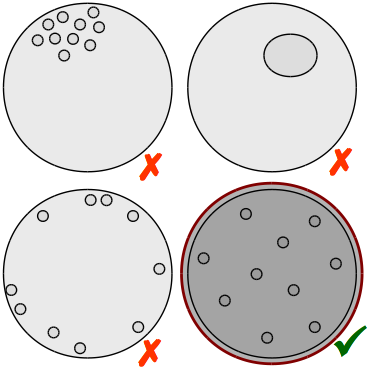
\includegraphics[scale=.5]{sample.png}
    \column{.5\textwidth}
        \pause
        \begin{items}
            \item If it is representative, I can generalize
            \pause
            \item Need a method of generating very random configurations from the 
                        feature model
        \end{items}
    \end{columns}
\end{frame}

\begin{frame}[t]{Research Questions - Revisited}

    \begin{items}
        \item How many bugs?
        \item What are the most common types of bugs?
        \item Where are most bugs?
        \item Which features are error-prone?
        \pause
        \item \color{red}{... Additional questions?}
        \item \color{red}{... Prioritization?}
        \item \color{red}{... Take a few minutes to brainstorm about it}
    \end{items}
    
    \begin{items}
        \item \color{gray}{(One-disabled vs. randconfig)}
    \end{items}
\end{frame}

\begin{frame}[t]{Methodology}


    \begin{columns}[T]
    \column{.5\textwidth}
        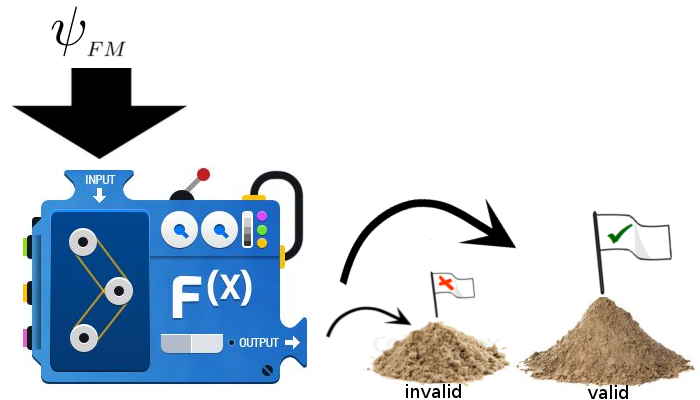
\includegraphics[scale=.5]{machine.png}
    \column{.5\textwidth}
        \begin{items}
            \item Feed it with the feature model
            \pause
            \item Collect $\kappa_{random}$
            \pause
            \item Assure $\kappa_{random} \in \mathbb{K}$
        \end{items}
    \end{columns}
\end{frame}
    

\begin{frame}[t]{Methodology}

    \begin{columns}[T]
    \column{.33\textwidth}
        \textbf{Exploit existing randconfig}
        % Introduction to randconfig
        % Flip a coin for every feature
        % Will look at dependencies first
        % Designed for Testing purpose
        % They have maybe not laid much work in on this
        \pause
        \begin{items}
            \item Concatenate Kconfig files
            \item Permute the order
            \item Flatten the structure
            \pause
            \item Run \emph{randconfig}
            \pause
            \item Still biased in the coin flipping !
            \pause
            \item See following Kconfig example
        \end{items}
    \column{.33\textwidth}
    \column{.33\textwidth}
    \end{columns}

\end{frame}

\begin{frame}[t,fragile]{randconfig bias}

    \begin{columns}[T]
    \column{.3\textwidth}
    \begin{Verbatim}
config A
    bool

config B
    bool
    depends on A
    \end{Verbatim}

    \pause
    \column{.6\textwidth}

    \begin{items}
        \item Possible configurations with \emph{randconfig}'s probabilities  are:
        \begin{items}
            \item () \textbf{\emph{50\%}}
            \item (A) \textbf{\emph{25\%}}
            \item (A,B) \textbf{\emph{25\%}}
        \end{items}
        \pause
        \item This is biased, and not representative.
    \end{items}

    \end{columns}
\end{frame}

\begin{frame}[t,fragile]{randconfig bias}

    \begin{columns}[T]
    \column{.3\textwidth}

    \begin{Verbatim}
config A
    bool

config B
    bool
    depends on A
    \end{Verbatim}

    \column{.6\textwidth}

    \begin{items}
        \item We would prefer a totally equal probability:
        \begin{items}
            \item () \textbf{\emph{33\%}}
            \item (A) \textbf{\emph{33\%}}
            \item (A,B) \textbf{\emph{33\%}}
        \end{items}
        \pause
        \item And so maybe we could invent something
    \end{items}

    \end{columns}
\end{frame}

\begin{frame}[t]{Methodology}

    \begin{columns}[T]
    \column{.33\textwidth}
        \color{lightgray}{
        \textbf{Exploit existing randconfig}
        % Introduction to randconfig
        % Flip a coin for every feature
        % Will look at dependencies first
        % Designed for Testing purpose
        % They have maybe not laid much work in on this
        \begin{items}
        \color{lightgray}{
            \item Concatenate Kconfig files
            \item Permute the order
            \item Flatten the structure
            \item Run \emph{randconfig}
            \item Still biased in the coin flipping !
            \item See following Kconfig example
        }
        \end{items}
        }
    \column{.33\textwidth}
        \textbf{Invent elvisconfig}
        \begin{items}
            \item Same idea as \emph{randconfig}
            \pause
            \item Try to fix bias in coin flipping
            \pause
            \item Need to know \#configs(A) vs. \#configs($\neg$A)
            \pause
            \item May be impossible
        \end{items}
    \column{.33\textwidth}
    \end{columns}

\end{frame}


\begin{frame}[t]{Methodology}

    \begin{columns}[T]
    \column{.33\textwidth}
        \color{lightgray}{
        \textbf{Exploit existing randconfig}
        % Introduction to randconfig
        % Flip a coin for every feature
        % Will look at dependencies first
        % Designed for Testing purpose
        % They have maybe not laid much work in on this
        \begin{items}
        \color{lightgray}{
            \item Concatenate Kconfig files
            \item Permute the order
            \item Flatten the structure
            \item Run \emph{randconfig}
            \item Still biased in the coin flipping !
            \item See following Kconfig example
        }
        \end{items}
        }
    \column{.33\textwidth}
        \color{lightgray}{
        \textbf{Invent elvisconfig}
        \begin{items}
        \color{lightgray}{
            \item Same idea as \emph{randconfig}
            \item Try to fix bias in coin flipping
            \item Need to know \#configs(A) vs. \#configs($\neg$A)
            \item May be impossible
        }
        \end{items}
    }
    \column{.33\textwidth}
        \textbf{Generate 'n' Filter}
        \begin{items}
            \item Flip a coin for every feature
            \pause
            \item Do not visit dependencies
            \pause
            \item Check for validity
            \pause
            \begin{items}
                \item Kconfig tool
                \item SAT checker
            \end{items}
            \pause
            \item Uniform distribution
            \pause
            \item May take much time
        \end{items}
    \end{columns}

\end{frame}

\begin{frame}[t]{Methodology}

    \begin{columns}[T]
    \column{.33\textwidth}
        \textbf{Exploit existing randconfig}
        % Introduction to randconfig
        % Flip a coin for every feature
        % Will look at dependencies first
        % Designed for Testing purpose
        % They have maybe not laid much work in on this
        \begin{items}
        \color{lightgray}{
            \item Concatenate Kconfig files
            \item Permute the order
            \item Flatten the structure
            \item Run \emph{randconfig}
            \item Still biased in the coin flipping !
            \item See following Kconfig example
        }
        \end{items}
    \column{.33\textwidth}
        \textbf{Invent elvisconfig}
        \begin{items}
        \color{lightgray}{
            \item Same idea as \emph{randconfig}
            \item Try to fix bias in coin flipping
            \item Need to know \#configs(A) vs. \#configs($\neg$A)
            \item May be impossible
        }
        \end{items}
    \column{.33\textwidth}
        \textbf{Generate 'n' Filter}
        \begin{items}
        \color{lightgray}{
            \item Flip a coin for every feature
            \item Do not visit dependencies
            \item Check for validity
            \begin{items}
            \color{lightgray}{
                \item Kconfig tool
                \item SAT checker
            }
            \end{items}
            \item Uniform distribution
            \item May take much time
        }
        \end{items}
    \end{columns}


    \begin{center}
    \textbf{\color{red}{Other ideas? Best solution?}}
    \end{center}

\end{frame}


\begin{frame}[t]{Analysing - Data collection}

    \begin{items}
        \item Analyse one random configuration \pause(with \textbf{gcc})
        \pause
        \item Save all kinds of information
        \begin{items}
            \item Configuration.
            \pause
            \item Errors / warnings
            \pause
            \item Program versions (Linux / gcc)
            \pause
            \item Make a bug reproducable
        \end{items}
        \pause
        \item Do it over and over again (with a new random configuration)
    \end{items}


\end{frame}

\begin{frame}[t]{Kconfig}

    \begin{items}
        \item The language of the feature model in Linux \color{gray}{(Busybox and others)}
        \pause
        \begin{items}
            \item Grammar
            \item Data types
            \item Transformation
        \end{items}

    \end{items}
\end{frame}

\begin{frame}[t,fragile]{Kconfig - Grammar}
    \begin{Verbatim}
K ->      "config" ID TYPE OPT*
        | "if" ID K "endif"
        | "choice" K+ "endchoice"

TYPE ->   "bool" | "tristate" | "string" | "int"

OPT  ->   "default" STRING
        | "range" INT
        | "depends on" ID
        | "select" ID
    \end{Verbatim}
\end{frame}

\begin{frame}[t,fragile]{Kconfig - Data types}
    \begin{columns}[T]
    \column{.5\textwidth}
    \begin{Verbatim}
config A
    \textbf{bool}
config B
    \textbf{tristate}
config C
    \textbf{int}
    range 5 15
config D
    \textbf{hex}
    default "c0000000"
config E
    \textbf{string}
    default "FOO"
    \end{Verbatim}
    \column{.5\textwidth}
    \begin{Verbatim}

y (ENABLED), n (DISABLED)

y, n, module

integers 


hexadecimals 


string
    \end{Verbatim}
    \end{columns}
\end{frame}

\begin{frame}[t,fragile]{Kconfig - Transformation}
    \begin{columns}[c]
    \column{.3\textwidth}
    \begin{Verbatim}
config A
    bool

\textbf{if A}
    config B
        bool
    
    config C
        bool
\textbf{endif}
    \end{Verbatim}

    \column{.3\textwidth}
    
\includegraphics[scale=.3]{arrowright.png}

    \textbf{Transformation}
    

    \column{.3\textwidth}
    \begin{Verbatim}
config A
    bool

config B
    bool
    \textbf{depends on A}

config C
    bool
    \textbf{depends on A}
    \end{Verbatim}
    \end{columns}
\end{frame}

\begin{frame}[t,fragile]{Threats to validity}

    \begin{columns}[T]
    \column{0\textwidth}

    \begin{Verbatim}
    
    \end{Verbatim}

    \column{1\textwidth}

    \begin{items}
        \item Sample not being representative
        \item Not getting enough bugs
        \pause
        \item \color{red}{Can you think of more?}
    \end{items}

    \end{columns}
\end{frame}

\begin{frame}[t]{Bye}
    \begin{center}
        Thank you for your time.
    \end{center}
\end{frame}

\end{document}
